\chapter{Особенности систем электронных голосований}

В настоящее время проведение демократических голосования является основной процедурой для решения общественно важный вопросов. Самым распространённым методом проведения голосований является бумажная система. Данный метод проведения обладает такими недостатками, как возможности для фальсификаций, возможные ошибки подсчета, высокая экономическая стоимость, отсутствие прозрачности процедуры проведения. Однако, классические электронные системы не получили распространения в виду проблем с безопасностью, конфиденциальностью, прозрачности программного обеспечения.

\section{Технология блокчейн, как решение большинства существующих проблем систем голосования}

Основываясь на описанной в первой главе информации о блокчейне, можно считать следующие преимущества использования этой технологии в процессе электронного голосования:

\begin{enumerate} 
  \item Анонимность избирателя, благодаря алгоритму слепой подписи, основанного на сложности факторизации больших составных чисел.
  
  \item Прозрачность процесса голосования, поскольку любой человек сможет развернуть узел с полной копией данных, а внесение изменений в состояние требует консенсуса среди большинства узлов.
  
  \item Подлинность результатов, так как любой человек сможет проверить какое число избирателей могло принимать участие в голосовании, кто из них получил подпись и отдал свой голос, а кто нет.
\end{enumerate}

Самый простой способ реализовать систему электронных голосований на базе блокчейна — это развернуть смарт-контракт на уже существующей публичной блокчейн платформе, который позволит организаторам создавать голосования, а избирателям отдавать свои голоса за кандидатов.

\section{Простейший протокол тайного электронного голосования}

Простейший алгоритм тайного электронного голосования по своей сути является перепиской с электронными подписями между избирателями и валидатором. Пусть \verb|V| (validator) — валидатор, проводящий электронное голосование, \verb|E| (elector) — избиратель, \verb|B| (ballot) — выбор избирателя. Процесс голосования с использованием данного протокола выглядит следующим образом:

\begin{enumerate} 
  \item \verb|V| публикует списки зарегистрированных избирателей.
  
  \item \verb|V| генерирует открытый и закрытый ключ, выкладывает открытый ключ в общим доступ. Любой может зашифровать свое сообщение при помощи опубликованного публичного ключа, однако расшифровать его сможет только \verb|V|.
  
  \item \verb|E| создает собственный открытый и закрытый ключ, выкладывает открытый ключ в общий доступ. Любой может проверить, что отправленное сообщение принадлежит \verb|E|, при помощи открытого ключа, однако подписать сообщение может только \verb|E|, при помощи закрытого ключа.
  
  \item \verb|E| формирует сообщение \verb|B|, подписывает это сообщение своим закрытым ключом, шифрует сообщение открытым ключом, и отправляет шифрованное сообщение \verb|V|.
  
  \item \verb|V| с помощью открытого ключа проверяет, что сообщение отправлено от зарегистрированного избирателя, расшифровывает сообщение своим закрытым ключом, добавляет выбор избирателя в общий подсчет.
\end{enumerate}

Данный протокол обеспечивает защиту от внешнего вмешательства, однако имеет очевидные недостатки, избирателям приходится полностью доверять валидатору, поскольку его работа никак не контролируется. Данный протокол используется только в том случае, когда все избиратели доверяют друг другу и организатору, отвечающему за сбор и подсчет голосов.

\section{Протокол электронного голосования Фудзиоки — Окамото — Оты}

В данном протоколе используется маскирующее (ослепляющие) шифрование. Маскирующие шифрование — особый вид шифрования, который дает возможность удостоверится в том, что документ подлинный и подписан авторизованным пользователем, однако, не дает узнать зашифрованные данные.

Для работы данного протокола используется заранее выбранный способ маскирующего шифрования, под которым избиратель отправляет свой выбор валидатору, так как маскирующие шифрование должно быть коммутативным с электронной подписью (формула (\ref{eq:sign})).
\begin{equation}\label{eq:sign}
sign(blind(B))=blind(sign(B))
\end{equation}
где  $B$ — сообщение с решением избирателя.

В общем случае, алгоритм слепой подпись выглядит следующим образом:

\begin{enumerate} 
  \item Избиратель зашифровывает сообщение $m$ функцией $f$, получая сообщение \(c=f(m)\).
  
  \item Избиратель отсылает зашифрованное сообщение валидатору.
  
  \item Валидатор вслепую подписывает сообщение c функцией $g$, получая \(c'=g(c)=g(f(m))\).
  
  \item Валидатор отсылает подписанное сообщение обратно избирателю.
  
  \item Избиратель убирает шифрование, получая \(c''=g(f(m))*f^{-1}=g(m)\).
\end{enumerate}

Данный алгоритм схематично представлен на рисунке \ref{fig:masksign}.

\begin{figure}[H]
\begin{center}
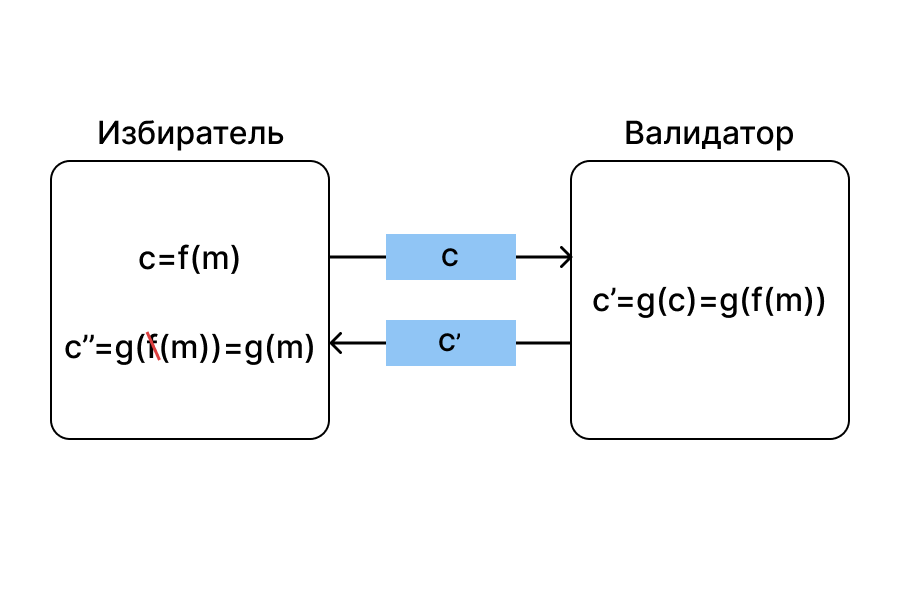
\includegraphics[width=0.9\hsize]{fig/mask-sign.png}\\[2mm]
\caption{Алгоритм слепой подписи}\label{fig:masksign}
\end{center}
\end{figure}

Пусть \verb|V| (validator) — регистратор, \verb|E| (elector) — избиратель, \verb|B| (ballot) — выбор избирателя, \verb|A| (agency) — агентство, проводящее голосование. Процесс голосования с использованием данного протокола выглядит следующим образом:

\begin{enumerate} 
  \item \verb|V| публикует списки зарегистрированных избирателей.
  
  \item \verb|V| генерирует открытый \(v_{public}\) и закрытый ключ \(v_{private}\), выкладывает открытый ключ в общим доступ. С помощью открытого ключа, любой может убедится, что сообщение подписано \verb|V|.
  
  \item \verb|E| создает собственный открытый \(e_{public}\) и закрытый ключ \(e_{private}\).
  
  \item \verb|E| формирует сообщение \verb|B|, шифрует это сообщение своим открытым ключом, накладывает на сообщение маскирующее шифрование \(blind(encrypt(e_{public}, B))\) и отправляет \verb|V|.
  
  \item \verb|V| проверяет, что сообщение отправлено от зарегистрированного избирателя, который еще не голосовал, подписывает его своим приватным ключом \(v_{private}\) и возвращает \verb|E|.
  
  \item \verb|E| снимает с сообщение слой маскирующего шифрования (в силу коммутативности остается \(sign(e_{private}, encrypt(e_{public}, B))\) и отправляет сообщение \verb|A|.
  
  \item После окончания голосования, \verb|E| отсылает \verb|A| свой приватный ключ \(e_{private}\).
  
  \item \verb|A| расшифровывает сообщения и подсчитывает результаты.  
\end{enumerate}

Данный протокол является одним из самых проверенных протоколов дистанционного голосования, он и его различные модификации чаще всего используется для проведения голосований.

\section{Внедрение блокчейна в процесс электронного голосования}

За основу данного протокола взят «Протокол Фудзиоки — Окамото — Оты». Субъекты, участвующие в процессе голосования: \verb|V| (validator) — организатор голосования, \verb|P| (platform) — платформа для проведения голосований, на технологии блокчейн, \verb|E| (elector) — избиратель, \verb|B| (ballot) — выбор избирателя. Процесс голосования выглядит следующим образом:

\begin{enumerate} 
  \item \verb|V| публикует списки зарегистрированных избирателей.
  
  \item \verb|V| генерирует открытый \(v_{public}\) и закрытый ключ \(v_{private}\), выкладывает открытый ключ в общим доступ. С помощью открытого ключа, любой может убедится, что сообщение подписано \verb|V|.
  
  \item \verb|V| создает голосование на платформе \verb|P|, передавая свой открытый ключ, количество зарегистрированных избирателей, дату и время начала голосования, дату и время окончания голосования, дату и время окончания принятия ключе расшифровки.
  
  \item \verb|E| создает собственный открытый \(e_{public}\) и закрытый ключ \(e_{private}\).
  
   \item \verb|E| формирует сообщение \verb|B|, шифрует это сообщение своим открытым ключом, накладывает на сообщение маскирующее шифрование \(blind(encrypt(e_{public}, B))\) и отправляет \verb|V|.
  
  \item \verb|V| проверяет, что сообщение отправлено от зарегистрированного избирателя, который еще не голосовал, подписывает его своим приватным ключом \(v_{private}\) и возвращает \verb|E|.
  
  \item \verb|E| снимает с сообщение слой маскирующего шифрования (в силу коммутативности остается \(sign(e_{private}, encrypt(e_{public}, B))\) и отправляет сообщение \verb|P|.
  
  \item \verb|P| проверяет, что подпись валидатора верна, записывает выбор избирателя в блокчейн.
  
   \item \verb|E| получает, в ответ на отправленную транзакцию, сообщение о том, что транзакция успешно завершена, после чего сразу же отправляет \verb|B| свой секретный ключ \(e_{private}\).
   
   \item \verb|B| проверяет, что выбор к которому добавляется секретный ключ \(e_{private}\), принадлежит \verb|E|, добавляет секретный ключ \(e_{private}\) к выбору \verb|E|.
   
   \item После окончания голосования, \verb|V| расшифровывает все бюллетени и подсчитывает голоса.
\end{enumerate}

Более наглядно процесс электронного голосования, согласно данному протоколу, продемонстрирован в виде диаграмм последовательности на рисунках \ref{fig:voteOne}, \ref{fig:voteTwo}, \ref{fig:voteThree}.

\begin{figure}[H]
\begin{center}
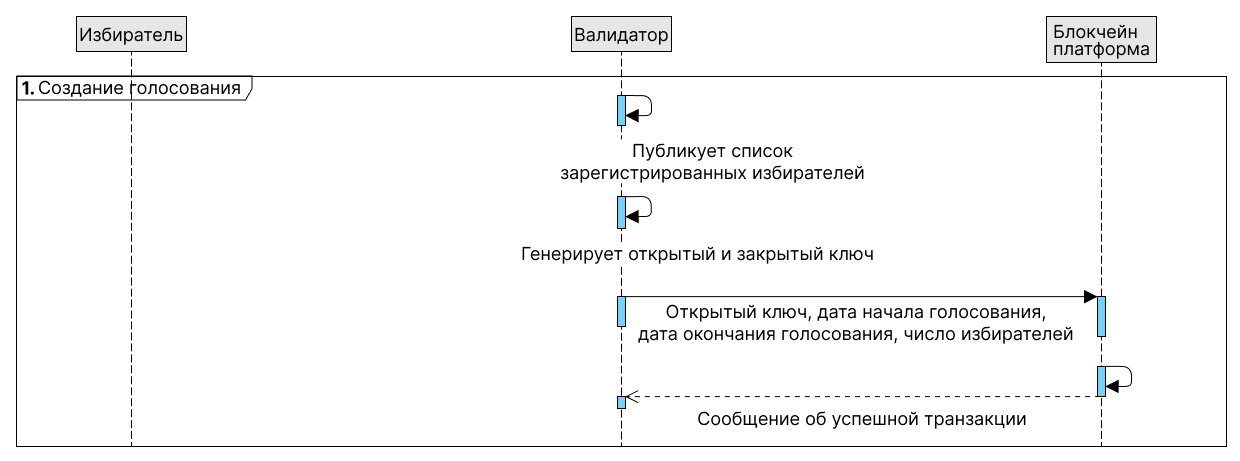
\includegraphics[width=1.0\hsize]{fig/nir-vote-1.png}\\[2mm]
\caption{Этап создания голосования}\label{fig:voteOne}
\end{center}
\end{figure}

\begin{figure}[H]
\begin{center}
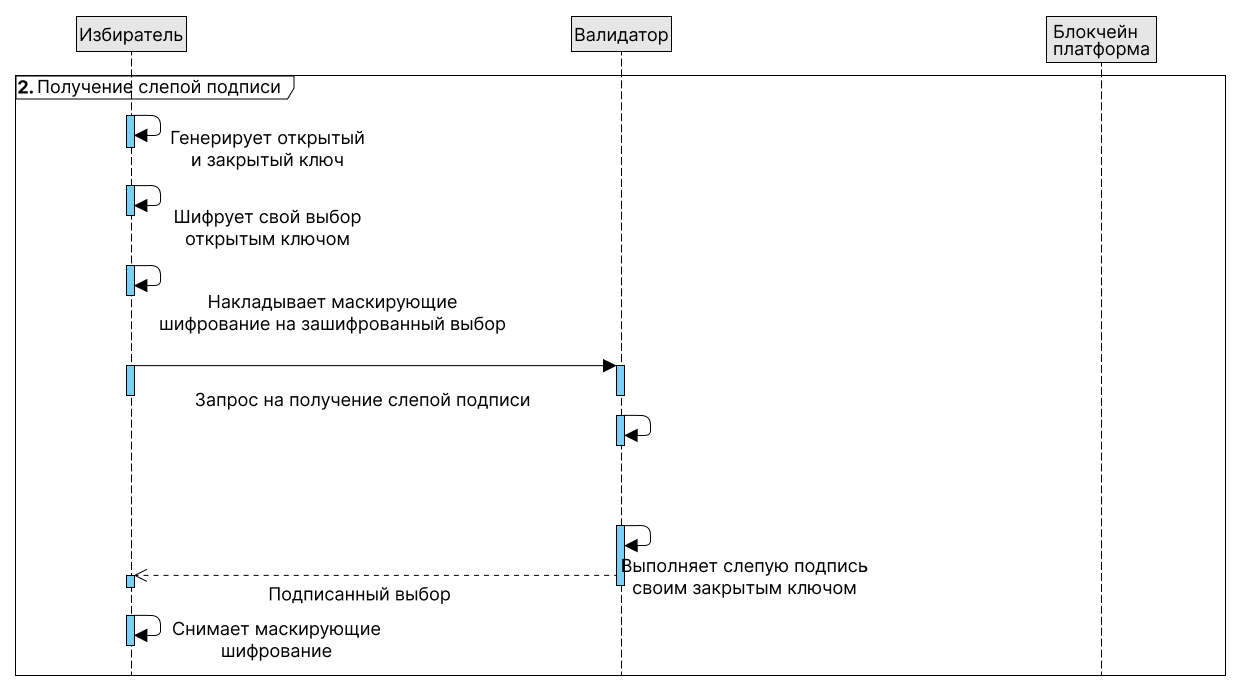
\includegraphics[width=1.0\hsize]{fig/nir-vote-2.png}\\[2mm]
\caption{Этап получения слепой подписи}\label{fig:voteTwo}
\end{center}
\end{figure}

\begin{figure}[H]
\begin{center}
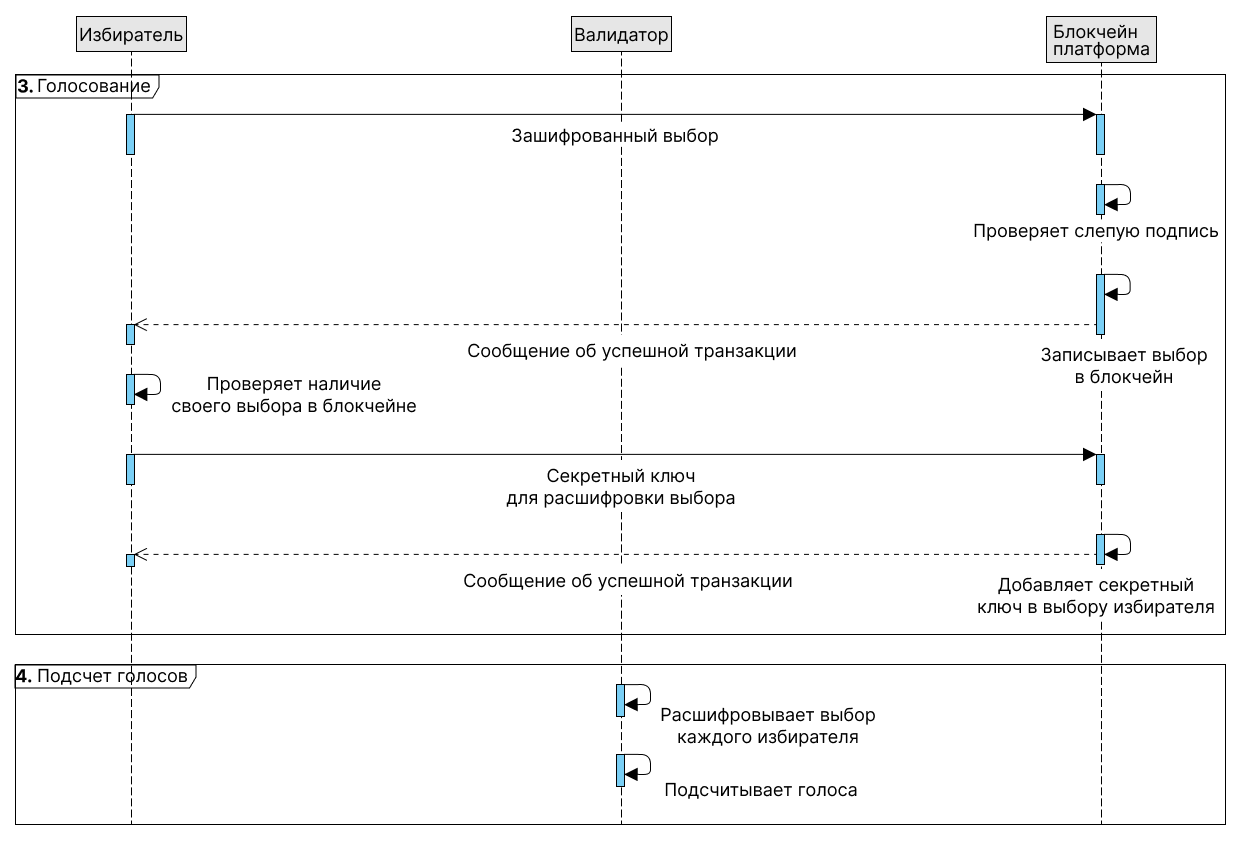
\includegraphics[width=1.0\hsize]{fig/nir-vote-3.png}\\[2mm]
\caption{Этап голосования и подсчета голосов}\label{fig:voteThree}
\end{center}
\end{figure}
